\section{Languages and Equivalence}
\label{sec:lang-eqdef}

\subsection{The \SpecL{} Language}
\label{sec:speclang}
We start with a discussion on the \SpecL{} language.
\SpecL{} supports recursive algebraic data types (ADT) similar to the ones available in most functional languages.
Additionally, \SpecL{} is equipped with the following scalar types: \type{Unit}, Boolean (\type{Bool}) and Bitvector of length N (\type{i<N>}).
ADTs can be thought of as `sum of product' types where each constructor represents a variant
and the arguments to each constructor represents its fields.
Evidently, types in \SpecL{} can be represented in {\em first order recursive types} with {\tt Product} and {\tt Sum} type constructors and {\tt Unit, Bool, i<N>} types (i.e., nullary type constructors) as follows:

$T \rightarrow {\tt \mu} \alpha.\ T \ |\  {\tt Product}(T,\dots,T) \ |\  {\tt Sum}(T,\dots,T) \ |\  {\tt Unit} \ |\ {\tt Bool} \ |\  {\tt i\langle N \rangle} \ |\  \alpha$

For example, the {\tt List} type can be written as $\mu \alpha. Sum(Unit, Product(i32,\alpha))$.

The language also borrows its expression grammar heavily from functional languages.
This includes the usual constructs like {\tt let-in}, {\tt if-then-else}, function application and the {\tt match} statement
for pattern-matching (i.e. deconstructing) sum and product values.
Unlike functional languages, \SpecL{} only supports first order functions.
Also, \SpecL{} does not support partial function application.
Hence, we constrain our attention to C programs containing only first order functions.
\SpecL{} is equipped with a special {\tt assuming-do} construct for explicitly providing assertions.
\SpecL{} also provides the typical boolean and bitvector operators for expressing computation in C succintly yet explicitly.
This includes logical operators (e.g., {\tt and}), bitvector arithmatic operators (e.g., {\tt bvadd(+)}) and
relational operators for comparing bitvectors interpreted as signed or unsigned integers (e.g., {\tt $\leq_{u,s}$}).

\begin{figure}[H]
\begin{small}
\begin{tabular}{rcl}
\nonTerm{expr} & $\rightarrow$ & \term{if} \nonTerm{expr} \term{then} \nonTerm{expr} \term{else} \nonTerm{expr} \\
& $|$ & \term{let} \nonTerm{id} \term{=} \nonTerm{expr} \term{in} \nonTerm{expr} \\
& $|$ & \term{match} \nonTerm{expr} \term{with} \nonTerm{match-clause-list} \\
& $|$ & \term{assuming} \nonTerm{expr} \term{do} \nonTerm{expr} \\
& $|$ & \nonTerm{id} \term{(} \nonTerm{expr-list} \term{)} \\
& $|$ & \nonTerm{data-cons} \term{(} \nonTerm{expr-list} \term{)} \\
& $|$ & \nonTerm{expr} \term{is} \nonTerm{data-cons} \\
& $|$ & \nonTerm{expr} \nonTerm{scalar-op} \nonTerm{expr} \\
& $|$ & \nonTerm{literal$_{\mathrm{Unit}}$} $|$ \nonTerm{literal$_{\mathrm{Bool}}$} $|$ \nonTerm{literal$_{\mathrm{i<N>}}$} \\
\\
\nonTerm{match-clause-list} & $\rightarrow$ & \nonTerm{match-clause}$^*$ \\
\nonTerm{match-clause} & $\rightarrow$ & \term{$|$} \nonTerm{data-cons} \term{(} \nonTerm{id-list} \term{)} \term{$\Rightarrow$} \nonTerm{expr} \\
\nonTerm{expr-list} & $\rightarrow$ & \term{$\epsilon$} \term{$|$} \nonTerm{expr} \term{,} \nonTerm{expr-list} \\
\nonTerm{id-list} & $\rightarrow$ & \term{$\epsilon$} \term{$|$} \nonTerm{id} \term{,} \nonTerm{id-list} \\
\\
\nonTerm{literal$_{\mathrm{Unit}}$} & $\rightarrow$ & \term{()} \\
\nonTerm{literal$_{\mathrm{Bool}}$} & $\rightarrow$ & \term{false} $|$ \term{true} \\
\nonTerm{literal$_{\mathrm{i<N>}}$} & $\rightarrow$ & [\term{0$\dots$2$^{\mathrm{N}}$-1}] \\
\end{tabular}
\end{small}
\caption{\label{fig:specgrammar}Simplified expression grammar of \SpecL{} language}
\end{figure}

\subsection{Intermediate Representations}
\label{sec:ir}
As summarized in \cref{sec:summary}, we lower both \SpecL{} and C programs to a common
intermediate representation (IR) for comparison.
IR is a Three-Address-Code (3AC) style intermediate representation.
We often omit intermediate registers in the IR for brevity and ease of exposition,
and refer to this as the {\em abstracted} IR.

\begin{figure}
\begin{tabular}{cc}
\begin{subfigure}[b]{0.45\textwidth}
\begin{center}
\begin{allLangEnvFoot}
~{\scriptsize \textcolor{mygray}{   }}~   
~{\scriptsize \textcolor{mygray}{S0:}}~ i32 sum_list (List l) {
~{\scriptsize \textcolor{mygray}{S1:}}~   i32 sum $\coloneqq$ ${\tt 0_{i32}}$;
~{\scriptsize \textcolor{mygray}{S2:}}~   while $\mathrm{\tt\neg (l\ is\ LNil)}$:
~{\scriptsize \textcolor{mygray}{S3:}}~     // (l is LCons);
~{\scriptsize \textcolor{mygray}{S4:}}~     sum $\coloneqq$ sum + ${\tt l.val}$;
~{\scriptsize \textcolor{mygray}{S5:}}~     l   $\coloneqq$ l.next;
~{\scriptsize \textcolor{mygray}{S6:}}~   return sum;
~{\scriptsize \textcolor{mygray}{SE:}}~ }
\end{allLangEnvFoot}
\end{center}
\caption{\label{fig:llTraverseSpec}(Abstracted) Spec IR}
\end{subfigure}%
&
\begin{subfigure}[b]{0.55\textwidth}
\begin{center}
\begin{allLangEnvFoot}
~{\scriptsize \textcolor{mygray}{\ \ \ }}~ unsigned sum_list (lnode* l);
~{\scriptsize \textcolor{mygray}{C0:}}~ i32 sum_list (i32 l) {
~{\scriptsize \textcolor{mygray}{C1:}}~   i32 sum $\coloneqq$ ${\tt 0_{i32}}$;
~{\scriptsize \textcolor{mygray}{C2:}}~   while ${\tt l \neq 0_{i32}}$:
~{\scriptsize \textcolor{mygray}{C3:}}~     sum $\coloneqq$ sum + $\structPointer{\tt l}{m}{\tt lnode}{val}$;
~{\scriptsize \textcolor{mygray}{C4:}}~     l   $\coloneqq$ $\structPointer{\tt l}{m}{\tt lnode}{next}$;
~{\scriptsize \textcolor{mygray}{C5:}}~   return sum;
~{\scriptsize \textcolor{mygray}{CE:}}~ }
\end{allLangEnvFoot}
\end{center}
\caption{\label{fig:llTraverseC}(Abstracted) C IR}
\end{subfigure}%
\\
\begin{subfigure}[b]{0.45\textwidth}
\begin{center}
{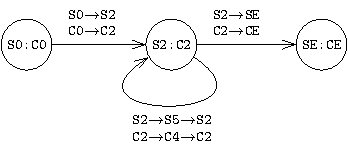
\includegraphics[scale=1.1]{chapters/figures/figSumListProductCfg.pdf}}
\end{center}
\caption{\label{fig:llTraverseProduct}Product-CFG}
\end{subfigure}%
&
\begin{subfigure}[b]{0.55\textwidth}
\begin{center}
\begin{footnotesize}
\begin{tabular}{|c|l|}
\hline
\tt PC-Pair & \multicolumn{1}{c|} {\tt Invariants} \\
\hline
\hline
${\tt (S0:C0)}$ &
\Tstrut ${\tt {\circled{P}}\  l_{S}\indEq{}Clist^{lnode}_{m}(l_{C})}$ \\
\multirow{2}{*}{${\tt (S2:C2)}$} &
\Tstrut \Bstrut ${\tt {\scriptsize \circled{I1}}\  l_{S}\indEq{}Clist^{lnode}_{m}(l_{C})}$ \\ & ${\tt {\scriptsize \circled{I2}}\  sum_{S}=sum_{C}}$ \\
${\tt (SE:CE)}$ &
\Tstrut \Bstrut ${\tt {\circled{E}}\  ret_{S}=ret_{C}}$ \\
\hline
\end{tabular}
\end{footnotesize}
\vspace{13px}
\end{center}
\caption{\label{fig:llTraverseProductInv}Node Invariants of the Product-CFG}
\end{subfigure}%
\\
\end{tabular}
\caption{\label{fig:llTraverseSpecAndC}Spec and C programs for traversing a linked list. \Cref{fig:llTraverseProduct} shows the Product-CFG between the IRs in \cref{fig:llTraverseSpec,fig:llTraverseC}. The inductive invariants of the Product-CFG are given in \cref{fig:llTraverseProductInv}.}
\end{figure}

\begin{figure}
\begin{tabular}{cc}
\begin{subfigure}[b]{0.45\textwidth}
\begin{center}
\begin{allLangEnvFoot}
~{\scriptsize \textcolor{mygray}{S0:}}~ i32 sum_list (List l) {
~{\scriptsize \textcolor{mygray}{S1:}}~   i32 sum $\coloneqq$ ${\tt 0_{i32}}$;
~{\scriptsize \textcolor{mygray}{S2:}}~   while $\neg$(l is LNil):
~{\scriptsize \textcolor{mygray}{S3:}}~     // (l is LCons);
~{\scriptsize \textcolor{mygray}{S4:}}~     sum $\coloneqq$ sum + l.val;
~{\scriptsize \textcolor{mygray}{S5:}}~     l   $\coloneqq$ l.next;
~{\scriptsize \textcolor{mygray}{S6:}}~   return sum;
~{\scriptsize \textcolor{mygray}{SE:}}~ }
\end{allLangEnvFoot}
\end{center}
\caption{\label{fig:llTraverseSpecIR}(Abstracted) Spec IR}
\end{subfigure}%
&
\begin{subfigure}[b]{0.55\textwidth}
\begin{center}
\begin{allLangEnvFoot}
~{\scriptsize \textcolor{mygray}{C0:}}~ i32 sum_list (i32 l) {
~{\scriptsize \textcolor{mygray}{C1:}}~   i32 sum $\coloneqq$ ${\tt 0_{i32}}$;
~{\scriptsize \textcolor{mygray}{C2:}}~   while ${\tt l \neq 0_{i32}}$:
~{\scriptsize \textcolor{mygray}{C3:}}~     sum $\coloneqq$ sum + $\structPointer{\tt l}{\mem{}}{lnode}{val}$;
~{\scriptsize \textcolor{mygray}{C4:}}~     l   $\coloneqq$ $\structPointer{\tt l}{\mem{}}{lnode}{next}$;
~{\scriptsize \textcolor{mygray}{C5:}}~   return sum;
~{\scriptsize \textcolor{mygray}{CE:}}~ }
\end{allLangEnvFoot}
\vspace{7px}
\end{center}
\caption{\label{fig:llTraverseCIR}(Abstracted) C IR}
\end{subfigure}%
\\
\begin{subfigure}[b]{0.45\textwidth}
\begin{center}
{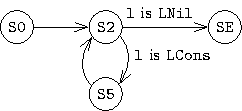
\includegraphics[scale=1.3]{chapters/figures/figSumListSpecCfg.pdf}}
\end{center}
\caption{\label{fig:llTraverseSpecCFG}CFG of \SpecL{} Program}
\end{subfigure}%
&
\begin{subfigure}[b]{0.55\textwidth}
\begin{center}
{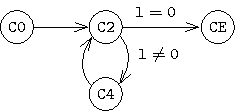
\includegraphics[scale=1.3]{chapters/figures/figSumListCCfg.pdf}}
\end{center}
\caption{\label{fig:llTraverseCCFG}CFG of C Program}
\end{subfigure}%
\\
\end{tabular}
\caption{\label{fig:llTraverseSpecAndCIRAndCFG}IRs and CFGs of the \SpecL{} and C Programs in \cref{fig:llTraverseSpec,fig:llTraverseC} respectively.}
\end{figure}


\Cref{fig:llTraverseSpec,fig:llTraverseC} show \SpecL{} and C programs that traverse a linked list
and return the sum of all the values in the linked list.
The corresponding IR programs are shown in \cref{fig:llTraverseSpecIR,fig:llTraverseCIR}.

During conversion of a \SpecL{} source (\cref{fig:llAllocSpec,fig:llTraverseSpec} resp.)
to IR (\cref{fig:llAllocSpecIR,fig:llTraverseSpecIR} resp.),
(a) {\tt match} statements are lowered to explicit \sumDtor{} conditionals where each branch
represents a distinct constructor,
(b) all tail-recursive calls are converted to loops while non-tail calls are preserved and
(c) all helper functions are inlined at their call-site.

Similarly, the following is performed during conversion of a C source (\cref{fig:llAllocC,fig:llTraverseC} resp.)
to IR (\cref{fig:llAllocCIR,fig:llTraverseCIR} resp.):
(a) the sizes and memory layouts of both scalar (e.g., \type{unsigned})
and compound (e.g., \type{struct lnode}) types are concretized,
(b) the program memory along with reads and writes to it are made explicit and
(c) we annotate {\tt malloc} calls with the call-site
i.e. IR PC (e.g., {\tt malloc$_\cpc{4}$} in \cref{fig:llAllocCIR}).

The IR supports both scalar and ADT types available in \SpecL{}.
Each ADT value is modeled as a key-value dictionary that maps
each of its field names to the constituent values.
These key-value pairs are accessed using the {\em accessor}-operator,
e.g., \prodAccess{l}{val} and \prodAccess{l}{next} represents the first and second
fields of the \cons{LCons} constructor in \cref{fig:llTraverseSpecIR}.
The IR also allows querying the top-level value constructor of an ADT value
using the {\em is}-operator, e.g., \sumIs{l}{LNil} in \cref{fig:llTraverseSpecIR}.
Importantly, $l.val$ is only well-formed if \sumIs{l}{LCons}.
The construction of the \SpecL{} IR ensures the well-formedness of all expressions.
Using the {\em accessor}- and {\em is}-operators, a \type{List} value $l$ can be expanded as:

\begin{equation}
\label{eqn:specDeconstruct}
U_S: l = \sumIf{\sumIs{l}{LNil}} \  \sumThen{\cons{LNil}} \  \sumElse{\cons{LCons}(\prodAccess{l}{val}, \prodAccess{l}{next})}
\end{equation}

In this expanded representation of $l$,
the {\em sum-deconstruction} operator `\sumDtor{}'
\footnote{The sum-deconstruction operator `\sumDtor{}' for an ADT
$T$ must contain exactly one branch for each value constructor of $T$.
For example, `\sumDtor{}' for the \type{List} type must have exactly two branches
of the form \cons{LNil} and $\cons{LCons}(e_1,e_2)$ for some expressions $e_1$ and $e_2$.}
conditionally deconstructs the sum type into its variants \cons{LNil} and \cons{LCons}.
\Cref{eqn:specDeconstruct} is called the {\em unrolling procedure} for the \type{List} variable $l$.
We can similarly define the unrolling procedure for any ADT variable.

Pointers are converted to bitvectors and the C memory 
is modeled as a byte-addressable array \mem{} in the IR.
Memory reads are represented using the following two C-like syntaxes:
(a) ``\structPointer{p}{\mem{}}{T}{f}'' is equivalent to ``*(\typeof{T.f}*)(\&\mem{}[$p$+\offsetof{T}{f}])''
i.e., it returns the bytes in the memory array \mem{} starting at address `$p$+\offsetof{T}{f}'
and interpreted as an object of type `\typeof{T.f}' and
(b) ``\arrIndex{p}{i}{\mem{}}{T}'' is equivalent to ``*(T*)(\&\mem{}[$p+i\times$\sizeof{T}])''
i.e., it returns the bytes in the memory array \mem{} starting at address `$p+i\times$\sizeof{T}'
and interpreted as an object of type `\type{T}'.
``\memWrite{\mem{}}{a}{v}{T}'' represents an array that is equal to \mem{} everywhere except at addresses
[$a$, $a$+\sizeof{T}) which contains the value $v$ of type `\type{T}'.

\Cref{fig:llTraverseSpecCFG,fig:llTraverseCCFG} show the Control-Flow Graph (CFG) representation
of the \SpecL{} and C IRs in \cref{fig:llTraverseSpecIR,fig:llTraverseCIR} respectively.
Each CFG node represents a IR PC location of the program and edges represent
transitions through execution of instructions.
Each edge is associated with:
(a) a {\em edge condition} (the condition under which that edge is taken),
(b) a {\em transfer function} (how the program state is mutated if that edge is taken) and
(c) a {\em UB assumption} (what condition should be true for the program execution
to be well-defined across this edge).
In \SpecL{}, assertions expressed using the {\tt assuming-do} statement
form the UB assumptions.
For brevity, we often represent a sequence of instructions with a single edge, e.g.,
in \cref{fig:llAllocCCFG}, the edge \cpath{5,3} represents the path \cpath{5,6,7,8,3}.
In such a case, the transfer function of the edge is the composition of the sequence of instructions.
Henceforth, We refer to the IR programs as \SpecL{} and C directly unless a distinction is necessary.

\subsection{Equivalence Definition}
\label{sec:eqdef}
Given (1) a \SpecL{} program specification $S$, (2) a C implementation $C$,
(3) a precondition $Pre$ that relates the initial inputs \sv{Input} and \cv{Input} to
$S$ and $C$ respectively, and (4) a postcondition $Post$ that relates the final outputs
\sv{Output} and \cv{Output} of $S$ and $C$ respectively\footnote{\cv{Input} and \cv{Output}
include the initial and final memory state of $C$ respectively.}:
$S$ and $C$ are {\em equivalent} if for all possible inputs \sv{Input} and \cv{Input} such that
$Pre(\sv{Input},\cv{Input})$ holds,
$S$'s execution is well-defined on \sv{Input}, {\em and}
$C$'s memory allocation requests during its execution on \cv{Input} are successful,
then both programs $S$ and $C$ produce outputs such that $Post(\sv{Output},\cv{Output})$ holds.
$$
Pre(\sv{Input},\cv{Input}) \land \sdef{} \land \cfits{} \Rightarrow Post(\sv{Output},\cv{Output})
$$

The \sdef{} antecedent states that we are only interested in proving equivalence for
well-defined executions of $S$, i.e., executions that satisfy all assertions expressed
using the {\tt assuming-do} statement.
Sometimes, the user may be interested in constraining the nature of inputs to $C$
for the purpose of checking equivalence only for {\em well-defined} inputs.
In these cases, we use a combination of $Pre$ and \sdef{} to constrain
the execution of $C$ to inputs for which we are interested in proving equivalence.
For example, the C library function {\tt strlen(\type{char}* \cv{str})} is well-defined only if \cv{str}
represents a valid null character terminated string.
This includes the assumption that the pointer \cv{str} may not be null.
Since \SpecL{} has no notion of pointers, we expose this conditional well-definedness of C strings
through an explicit constructor e.g. \cons{SInvalid} for the \type{String} ADT defined as
$\type{String}=\cons{SInvalid}\ |\ \cons{SNil}\ |\ \cons{SCons}(\type{i8}, \type{String})$.
\sdef{} asserts $\neg(\sumIs{\sv{str}}{SInvalid})$ and
the precondition $Pre$ contains the relation $(\sumIs{\sv{str}}{SInvalid}) \Leftrightarrow (\cv{str}=0)$.
Hence, \sdef{} and $Pre$ ensures that we compute equivalence only for those
executions of $S$ and $C$ where the input strings are well-defined.
A similar strategy is employed for other functions as detailed in \cref{sec:results}.

The \cfits{} antecedent states that we prove equivalence under the assumption that $C$'s memory
requirements fit within the available system memory i.e., only for those executions of $C$
in which all memory allocation requests (through {\tt malloc} calls) are successful.

The returned values of $S$ and $C$ procedures form their observable outputs.
For $S$, the returned values are explicit and may include ADT values.
For $C$, observables include the returned value along with the implicit memory state
at program exit.
The postcondition $Post$ relates these outputs of the two programs.
In general, the \SpecL{} and C sources may contain multiple procedures and these
procedures may have calls to each other.
In that scenario, we are interested in proving equivalence of each $S$ and $C$ procedure pair.

\begin{figure}
\begin{tabular}{cc}
\begin{subfigure}[b]{0.45\textwidth}
\begin{center}
{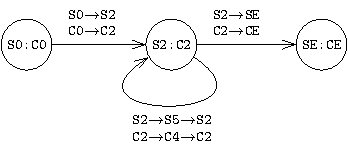
\includegraphics[scale=1.1]{chapters/figures/figSumListProductCfg.pdf}}
\end{center}
\caption{\label{fig:llTraverseProduct}Product-CFG}
\end{subfigure}%
&
\begin{subfigure}[b]{0.55\textwidth}
\begin{center}
\begin{footnotesize}
\begin{tabular}{|c|l|}
\hline
{\bf PC-Pair} & \multicolumn{1}{c|} {\bf Invariants} \\
\hline
\hline
(\scpc{0}{0}) &
\Tstrut $\circled{P}\  \sv{l} \indEq{} \lifted{list}{\mem{}}{lnode}{\cv{l}}$ \\
\multirow{2}{*}{(\scpc{2}{2})} &
\Tstrut $\circled{\scriptsize I1}\  \sv{l} \indEq{} \lifted{list}{\mem{}}{lnode}{\cv{l}}$ \\ &
\Tstrut $\circled{\scriptsize I2}\  \sv{sum} = \cv{sum}$ \\
(\scpc{E}{E}) &
\Tstrut $\circled{\scriptsize E}\  \sv{ret} = \cv{ret}$ \\
\hline
\end{tabular}
\end{footnotesize}
\vspace{13px}
\end{center}
\caption{\label{fig:llTraverseProductInv}Node Invariants of the Product-CFG}
\end{subfigure}%
\\
\end{tabular}
\caption{\label{fig:llTraverseProductCFGInvs} Product-CFG between the IRs in \cref{fig:llTraverseSpec,fig:llTraverseC}. The inductive invariants of the Product-CFG are given in \cref{fig:llTraverseProductInv}.}
\end{figure}


\subsection{Bisimulation Relation}
\label{sec:bisim}
We construct a {\em bisimulation relation} to identify equivalence between two programs.
A bisimulation relation correlates the transitions of $S$ and $C$ in lockstep, such that the
lockstep execution ensures identical observable behavior.
A bisimulation relation between two programs can be represented using a {\em product program}
\cite{covac} and the CFG representation of a product program is called a {\em product-CFG}.
\Cref{fig:llTraverseProduct} shows a product-CFG, that encodes the lockstep execution
(bisimulation relation) between the CFGs in \cref{fig:llTraverseSpecCFG,fig:llTraverseCCFG}.

A node in the product-CFG is formed by pairing nodes of $S$ and $C$ CFGs,
e.g., \scpc{2}{2} is formed by pairing \spc{2} and \cpc{2}.
If the lockstep execution of both programs is at node \scpc{2}{2} in the product-CFG,
then $S$'s execution is at \spc{2} and $C$'s execution is at \cpc{2}.
The start node \scpc{0}{0} of the product-CFG correlates the start nodes of CFGs of $S$ and $C$.
Similarly, the exit node \scpc{E}{E} correlates the exit nodes of both programs.

An edge in the product-CFG is formed by pairing a {\em path} (a sequence of edges) in $S$
with a path in $C$.
A product-CFG edge encodes the lockstep execution of its correlated paths.
For example, the product-CFG edge \scedge{2}{2}{2}{2} is formed by pairing
\spath{2,5,2} and \cpath{2,4,2} in \cref{fig:llTraverseSpecCFG,fig:llTraverseCCFG},
and represents that when $S$ makes the transition \spath{2,5,2}, $C$ makes the transition \cpath{2,4,2}
in lockstep.
In general, a product-CFG edge $e$ may correlate a finite path \sv{\rho} in $S$ with a finite path
\cv{\rho} in $C$, written $e=(\sv{\rho},\cv{\rho})$.
The empty path $\epsilon$ in $S$ may be correlated with a finite path in $C$
However, a product-CFG is only well-formed (i.e. represents a valid bisimulation relation)
if no loop path in $C$ is correlated with $\epsilon$ in $S$.
For example, \cref{fig:llAllocProductCFG} shows the correlation of
$\epsilon$ with the paths \cpath{3,4} and \cpath{4,5}.
Since the loop path \cpath{3,4,5,3} in $C$ is still correlated with
the non-empty path \spath{3,5,3} in $S$, it represents a valid bisimulation relation.

At the start node \scpc{0}{0} of the product-CFG in \cref{fig:llAllocProductCFG},
the precondition $Pre$ (labeled \circled{\small P})
ensures equality of input arguments \sv{n} and \cv{n} at programs' entry.
{\em Inductive invariants} (labeled \circled{\small I}) are inferred
at each intermediate product-CFG node that relate
the values of $S$ with values and memory state of $C$.
The inductive invariants are identified by running an invariant inference algorithm
on the product-CFG, which is further discussed in \cref{sec:invinference}.
At the exit node \scpc{E}{E} of the product-CFG, the postcondition $Post$ (labeled \circled{\small P})
represents equality of observable outputs and forms our primary proof obligation.
Assuming that the precondition $Pre$ (\circled{\small P}) holds at the entry node \scpc{0}{0},
a bisimulation check involves checking that the inductive invariants (\circled{\small I}) hold too,
and consequently the postcondition $Post$ (\circled{\small E}) holds at the exit node \scpc{E}{E}.

\subsection{Recursive Relation}
\label{sec:recrel}
In \cref{fig:llTraverseProductInv}, the precondition (\circled{\small P}) is an example
of a {\em \recursiveRelation{}}:
``\sv{l} \indEq{} \lifted{list}{\mem{}}{lnode}{\cv{l}}'' where \sv{l} and \cv{l}
represent the input variables to the \SpecL{} and C programs respectively,
\type{lnode} is the C \type{struct} type that contains the \field{val} and \field{next} fields,
and \mem{} is the byte-addressable array representing the current memory state of the C program.
$l_1 \indEq{} l_2$ is read {\em $l_1$ is recursively equal to $l_2$} and is semantically equivalent
to $l_1 = l_2$. The `\indEq{}' simply emphasizes that $l_1$ and $l_2$ are (possibly recursive) ADT values.
\lift{list}{}{lnode} is called a {\em lifting constructor} that `lifts' a C pointer value $p$
(pointing to an object of type \type{struct lnode}) and
a C memory state \mem{} to a (possibly infinite in case of a circular list) \type{List} value,
and is defined through its {\em unrolling procedure} as follows:

\begin{equation}
\label{eqn:clist}
\begin{split}
U_C:\ &\lifted{list}{\mem{}}{lnode}{p \ctype{i32}} = \sumIf{p=0} \ \sumThen{\cons{LNil}} \\ & \qquad\qquad\ \ \ \sumElse{\cons{LCons}(\structPointer{p}{\mem{}}{lnode}{val}, \lifted{list}{\mem{}}{lnode}{\structPointer{p}{\mem{}}{lnode}{next}})}
\end{split}
\end{equation}

Note the recursive nature of the lifting constructor \lift{list}{}{lnode}: if the pointer $p$ is zero
(i.e. $p$ is a null pointer), then it represents the empty list \cons{LNil};
otherwise it represents the list formed by \cons{LCons}-ing the value stored at
\structPointer{p}{\mem{}}{lnode}{val} in memory \mem{} and the list formed by recursively
lifting \structPointer{p}{\mem{}}{lnode}{next} through \lift{list}{}{lnode}.
\lifted{list}{\mem{}}{lnode}{p} allows us to adapt a C linked list (formed by chasing a pointer $p$
in the memory \mem{}) to a \type{List} value and compare it with a \SpecL{} \type{List}
value for equality.

\subsection{Proof Obligations}
\label{sec:proofobl}
The counterexample-guided algorithms for construction of the product-CFG and inference of inductive
invariants are discussed later in \cref{sec:algo}.
For now, we discuss the proof obligations that arise from a given product-CFG.
Consider the product-CFG in \cref{fig:llAllocProductCFG}.
Recall that a bisimulation check involves checking that all inductive invariants
and the postcondition $Post$ hold at each product-CFG node.

We use relational Hoare triples to express these proof obligations \cite{relationalHoareLogic,hoareTriple}.
If $\phi$ denotes a predicate relating the machine states of $S$ and $C$, then
for a product-CFG edge $e=(\sv{\rho},\cv{\rho})$, \hoareTriple{\phi_s}{e}{\phi_d}
denotes the condition:
if any machine states \sv{\sigma} and \cv{\sigma} of programs $S$ and $C$ are related through
precondition $\phi_s(\sv{\sigma},\cv{\sigma})$ and the paths \sv{\rho} and \cv{\rho}
are executed in $S$ and $C$ respectively,
then execution terminates normally in states $\sv{\sigma}^{'}$ (for $S$) and
$\cv{\sigma}^{'}$ (for $C$) and postcondition $\phi_d(\sv{\sigma}^{'},\cv{\sigma}^{'})$ holds.

For every product-CFG edge $e = (s \rightarrow d) = (\sv{\rho}, \cv{\rho})$,
we are interested in proving: \hoareTriple{\phi_s}{\sv{\rho},\cv{\rho}}{\phi_d},
where $\phi_s$ and $\phi_d$ are the node invariants at the product-CFG nodes $s$ and $d$
respectively.
The weakest-precondition transformer is used to translate a Hoare triple
\hoareTriple{\phi_s}{\sv{\rho},\cv{\rho}}{\phi_d} to the following
first-order logic formula:

\begin{equation}
\label{eqn:firstOrderFormula}
(\phi_s \land pathcond_{\sv{\rho}} \land pathcond_{\cv{\rho}} \land ubfree_{\sv{\rho}}) \Rightarrow {\tt WP}_{{\sv{\rho},\cv{\rho}}}(\phi_d)
\end{equation}

Here, $pathcond_{\rho_X}$ represent the condition that path $\rho$ is taken in program $X$
and $ubfree_{\sv{\rho}}$ represents the condition that execution of $S$ along path $\sv{\rho}$
is free of undefined behaviour.
${\tt WP}_{{\sv{\rho},\cv{\rho}}}(\phi_d)$ represents the weakest-precondition
of the predicate $\phi_d$ across the product-CFG edge $e = (\sv{\rho},\cv{\rho})$.
We will use `\lhs{}' and `\rhs{}' to refer to the antecedent and consequent of
the implication operator `$\Rightarrow$' in \cref{eqn:firstOrderFormula}.

For example, checking that the loop invariant \circled{\small I2}
$\sv{l} \indEq{} \lifted{list}{\mem{}}{lnode}{\cv{l}}$ holds at \scpc{2}{2} in \cref{fig:llTraverseProduct}
requires us to prove the following two proof obligations:
\circled{1} \hoareTriple{\scpcinv{0}{0}}{\spath{0,2},\cpath{0,2}}{\sv{l} \indEq{} \lifted{list}{\mem{}}{lnode}{\cv{l}}} and
\circled{2} \hoareTriple{\scpcinv{2}{2}}{\spath{2,5,2},\cpath{2,4,2}}{\sv{l} \indEq{} \lifted{list}{\mem{}}{lnode}{\cv{l}}}.
The proof obligation \circled{2} reduces to the following first-order logic proof obligation:

\begin{equation}
\label{eqn:firstOrderFormulaExample}
\begin{split}
\sv{l} \indEq{} \lifted{list}{\mem{}}{lnode}{\cv{l}} \land \sv{sum} = \cv{sum}
\land (\sumIs{\sv{l}}{LCons}) \land (\cv{l} \neq 0) \\ \Rightarrow
\prodAccess{\sv{l}}{next} \indEq{} \lifted{list}{\mem{}}{lnode}{\structPointer{\cv{l}}{\mem{}}{lnode}{next}}
\end{split}
\end{equation}

Due to the presence of \recursiveRelations{}, these proof queries
(e.g., \cref{eqn:firstOrderFormulaExample}) cannot be solved directly by
off-the-shelf solvers and require special handling.
The next chapter illustrates our proof discharge algorithm for solving proof queries
involving \recursiveRelations{}.
